%% fig_minimalsupport.tex   (generated by make_round12.py; do not edit by hand)
%% Minimal support of a combination of natural objects at n = 4.
\documentclass[tikz,border=8pt]{standalone}
\usepackage{amsmath,amssymb}
\usetikzlibrary{arrows.meta,calc,decorations.pathreplacing}
%% palette.tex -- shared colour definitions for the figures
\definecolor{PInk}{RGB}{26,32,44}
\definecolor{PBlue}{RGB}{37,82,139}
\definecolor{PTeal}{RGB}{23,127,125}
\definecolor{POchre}{RGB}{193,138,44}
\definecolor{PClay}{RGB}{178,74,58}
\definecolor{PSlate}{RGB}{108,122,137}
\definecolor{PViolet}{RGB}{110,86,150}
\definecolor{WBlue}{RGB}{223,234,246}
\definecolor{WTeal}{RGB}{220,238,236}
\definecolor{WOchre}{RGB}{250,240,218}
\definecolor{WClay}{RGB}{247,229,224}
\definecolor{WSlate}{RGB}{238,241,244}
\definecolor{PMag}{RGB}{158,58,110}
\definecolor{PGrass}{RGB}{62,124,66}
\definecolor{PAmber}{RGB}{214,112,38}
\definecolor{PIndigo}{RGB}{58,64,140}
\definecolor{PRule}{RGB}{176,186,197}

%% shared macros so the standalone figures match the paper
\providecommand{\QQ}{\mathbb{Q}}
\providecommand{\ZZ}{\mathbb{Z}}
\providecommand{\RR}{\mathbb{R}}
\providecommand{\CC}{\mathbb{C}}
\providecommand{\PP}{\mathbb{P}}
\providecommand{\Kx}{K^{\times}}
\providecommand{\HW}{W}
\providecommand{\Nm}{\mathrm{N}}
\providecommand{\Hdg}{\mathrm{Hdg}}
\providecommand{\NS}{\mathrm{NS}}
\providecommand{\cA}{\mathcal{A}}
\providecommand{\cD}{\mathcal{D}}
\providecommand{\cF}{\mathcal{F}}
\providecommand{\cP}{\mathcal{P}}
\providecommand{\cO}{\mathcal{O}}
\providecommand{\cQ}{\mathcal{Q}}
\providecommand{\bbar}[1]{\overline{#1}}
\providecommand{\ch}{\operatorname{ch}}
\providecommand{\End}{\mathrm{End}}

\begin{document}
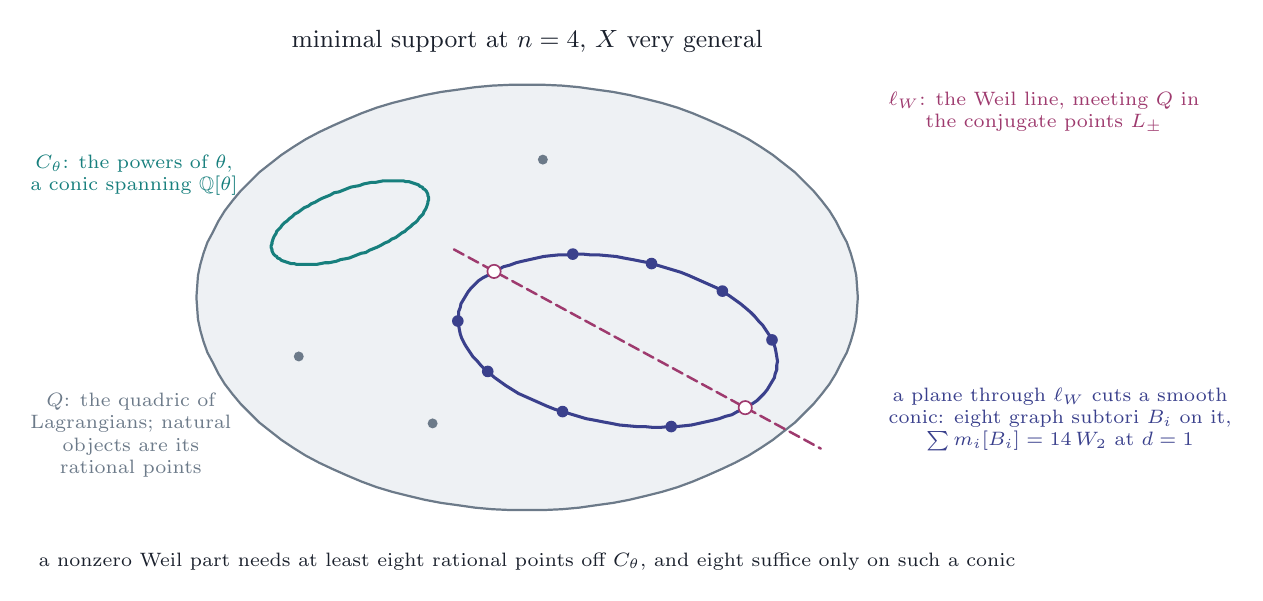
\begin{tikzpicture}[x=1cm,y=1cm,line join=round,line cap=round,
  font=\small,text=PInk]
  \fill[WSlate] plot[smooth cycle] coordinates {(4.20,0.00) (4.19,0.14) (4.18,0.28) (4.15,0.42) (4.11,0.56) (4.06,0.70) (3.99,0.83) (3.92,0.97) (3.84,1.10) (3.74,1.23) (3.64,1.35) (3.52,1.47) (3.40,1.59) (3.26,1.70) (3.12,1.81) (2.97,1.91) (2.81,2.01) (2.64,2.10) (2.47,2.18) (2.29,2.26) (2.10,2.34) (1.91,2.41) (1.71,2.47) (1.51,2.52) (1.30,2.57) (1.09,2.61) (0.87,2.64) (0.66,2.67) (0.44,2.69) (0.22,2.70) (0.00,2.70) (-0.22,2.70) (-0.44,2.69) (-0.66,2.67) (-0.87,2.64) (-1.09,2.61) (-1.30,2.57) (-1.51,2.52) (-1.71,2.47) (-1.91,2.41) (-2.10,2.34) (-2.29,2.26) (-2.47,2.18) (-2.64,2.10) (-2.81,2.01) (-2.97,1.91) (-3.12,1.81) (-3.26,1.70) (-3.40,1.59) (-3.52,1.47) (-3.64,1.35) (-3.74,1.23) (-3.84,1.10) (-3.92,0.97) (-3.99,0.83) (-4.06,0.70) (-4.11,0.56) (-4.15,0.42) (-4.18,0.28) (-4.19,0.14) (-4.20,0.00) (-4.19,-0.14) (-4.18,-0.28) (-4.15,-0.42) (-4.11,-0.56) (-4.06,-0.70) (-3.99,-0.83) (-3.92,-0.97) (-3.84,-1.10) (-3.74,-1.23) (-3.64,-1.35) (-3.52,-1.47) (-3.40,-1.59) (-3.26,-1.70) (-3.12,-1.81) (-2.97,-1.91) (-2.81,-2.01) (-2.64,-2.10) (-2.47,-2.18) (-2.29,-2.26) (-2.10,-2.34) (-1.91,-2.41) (-1.71,-2.47) (-1.51,-2.52) (-1.30,-2.57) (-1.09,-2.61) (-0.87,-2.64) (-0.66,-2.67) (-0.44,-2.69) (-0.22,-2.70) (-0.00,-2.70) (0.22,-2.70) (0.44,-2.69) (0.66,-2.67) (0.87,-2.64) (1.09,-2.61) (1.30,-2.57) (1.51,-2.52) (1.71,-2.47) (1.91,-2.41) (2.10,-2.34) (2.29,-2.26) (2.47,-2.18) (2.64,-2.10) (2.81,-2.01) (2.97,-1.91) (3.12,-1.81) (3.26,-1.70) (3.40,-1.59) (3.52,-1.47) (3.64,-1.35) (3.74,-1.23) (3.84,-1.10) (3.92,-0.97) (3.99,-0.83) (4.06,-0.70) (4.11,-0.56) (4.15,-0.42) (4.18,-0.28) (4.19,-0.14)};
  \draw[PSlate,line width=0.80pt] (4.20,0.00) -- (4.19,0.14) -- (4.18,0.28) -- (4.15,0.42) -- (4.11,0.56) -- (4.06,0.70) -- (3.99,0.83) -- (3.92,0.97) -- (3.84,1.10) -- (3.74,1.23) -- (3.64,1.35) -- (3.52,1.47) -- (3.40,1.59) -- (3.26,1.70) -- (3.12,1.81) -- (2.97,1.91) -- (2.81,2.01) -- (2.64,2.10) -- (2.47,2.18) -- (2.29,2.26) -- (2.10,2.34) -- (1.91,2.41) -- (1.71,2.47) -- (1.51,2.52) -- (1.30,2.57) -- (1.09,2.61) -- (0.87,2.64) -- (0.66,2.67) -- (0.44,2.69) -- (0.22,2.70) -- (0.00,2.70) -- (-0.22,2.70) -- (-0.44,2.69) -- (-0.66,2.67) -- (-0.87,2.64) -- (-1.09,2.61) -- (-1.30,2.57) -- (-1.51,2.52) -- (-1.71,2.47) -- (-1.91,2.41) -- (-2.10,2.34) -- (-2.29,2.26) -- (-2.47,2.18) -- (-2.64,2.10) -- (-2.81,2.01) -- (-2.97,1.91) -- (-3.12,1.81) -- (-3.26,1.70) -- (-3.40,1.59) -- (-3.52,1.47) -- (-3.64,1.35) -- (-3.74,1.23) -- (-3.84,1.10) -- (-3.92,0.97) -- (-3.99,0.83) -- (-4.06,0.70) -- (-4.11,0.56) -- (-4.15,0.42) -- (-4.18,0.28) -- (-4.19,0.14) -- (-4.20,0.00) -- (-4.19,-0.14) -- (-4.18,-0.28) -- (-4.15,-0.42) -- (-4.11,-0.56) -- (-4.06,-0.70) -- (-3.99,-0.83) -- (-3.92,-0.97) -- (-3.84,-1.10) -- (-3.74,-1.23) -- (-3.64,-1.35) -- (-3.52,-1.47) -- (-3.40,-1.59) -- (-3.26,-1.70) -- (-3.12,-1.81) -- (-2.97,-1.91) -- (-2.81,-2.01) -- (-2.64,-2.10) -- (-2.47,-2.18) -- (-2.29,-2.26) -- (-2.10,-2.34) -- (-1.91,-2.41) -- (-1.71,-2.47) -- (-1.51,-2.52) -- (-1.30,-2.57) -- (-1.09,-2.61) -- (-0.87,-2.64) -- (-0.66,-2.67) -- (-0.44,-2.69) -- (-0.22,-2.70) -- (-0.00,-2.70) -- (0.22,-2.70) -- (0.44,-2.69) -- (0.66,-2.67) -- (0.87,-2.64) -- (1.09,-2.61) -- (1.30,-2.57) -- (1.51,-2.52) -- (1.71,-2.47) -- (1.91,-2.41) -- (2.10,-2.34) -- (2.29,-2.26) -- (2.47,-2.18) -- (2.64,-2.10) -- (2.81,-2.01) -- (2.97,-1.91) -- (3.12,-1.81) -- (3.26,-1.70) -- (3.40,-1.59) -- (3.52,-1.47) -- (3.64,-1.35) -- (3.74,-1.23) -- (3.84,-1.10) -- (3.92,-0.97) -- (3.99,-0.83) -- (4.06,-0.70) -- (4.11,-0.56) -- (4.15,-0.42) -- (4.18,-0.28) -- (4.19,-0.14) -- (4.20,-0.00);
  \draw[PTeal,line width=1.10pt] (-1.26,1.31) -- (-1.27,1.33) -- (-1.28,1.35) -- (-1.30,1.37) -- (-1.32,1.38) -- (-1.33,1.40) -- (-1.36,1.41) -- (-1.38,1.43) -- (-1.41,1.44) -- (-1.44,1.45) -- (-1.47,1.46) -- (-1.50,1.47) -- (-1.54,1.47) -- (-1.57,1.48) -- (-1.61,1.48) -- (-1.65,1.48) -- (-1.70,1.48) -- (-1.74,1.48) -- (-1.79,1.48) -- (-1.83,1.48) -- (-1.88,1.47) -- (-1.93,1.46) -- (-1.98,1.46) -- (-2.03,1.45) -- (-2.08,1.44) -- (-2.13,1.42) -- (-2.19,1.41) -- (-2.24,1.40) -- (-2.29,1.38) -- (-2.34,1.36) -- (-2.39,1.34) -- (-2.45,1.33) -- (-2.50,1.30) -- (-2.55,1.28) -- (-2.60,1.26) -- (-2.64,1.24) -- (-2.69,1.21) -- (-2.74,1.19) -- (-2.78,1.16) -- (-2.83,1.14) -- (-2.87,1.11) -- (-2.91,1.08) -- (-2.95,1.06) -- (-2.98,1.03) -- (-3.02,1.00) -- (-3.05,0.97) -- (-3.08,0.95) -- (-3.11,0.92) -- (-3.13,0.89) -- (-3.16,0.86) -- (-3.18,0.84) -- (-3.19,0.81) -- (-3.21,0.78) -- (-3.22,0.76) -- (-3.23,0.73) -- (-3.24,0.70) -- (-3.24,0.68) -- (-3.25,0.66) -- (-3.25,0.63) -- (-3.24,0.61) -- (-3.24,0.59) -- (-3.23,0.57) -- (-3.22,0.55) -- (-3.20,0.53) -- (-3.18,0.52) -- (-3.17,0.50) -- (-3.14,0.49) -- (-3.12,0.47) -- (-3.09,0.46) -- (-3.06,0.45) -- (-3.03,0.44) -- (-3.00,0.43) -- (-2.96,0.43) -- (-2.93,0.42) -- (-2.89,0.42) -- (-2.85,0.42) -- (-2.80,0.42) -- (-2.76,0.42) -- (-2.71,0.42) -- (-2.67,0.42) -- (-2.62,0.43) -- (-2.57,0.44) -- (-2.52,0.44) -- (-2.47,0.45) -- (-2.42,0.46) -- (-2.37,0.48) -- (-2.31,0.49) -- (-2.26,0.50) -- (-2.21,0.52) -- (-2.16,0.54) -- (-2.11,0.56) -- (-2.05,0.57) -- (-2.00,0.60) -- (-1.95,0.62) -- (-1.90,0.64) -- (-1.86,0.66) -- (-1.81,0.69) -- (-1.76,0.71) -- (-1.72,0.74) -- (-1.67,0.76) -- (-1.63,0.79) -- (-1.59,0.82) -- (-1.55,0.84) -- (-1.52,0.87) -- (-1.48,0.90) -- (-1.45,0.93) -- (-1.42,0.95) -- (-1.39,0.98) -- (-1.37,1.01) -- (-1.34,1.04) -- (-1.32,1.06) -- (-1.31,1.09) -- (-1.29,1.12) -- (-1.28,1.14) -- (-1.27,1.17) -- (-1.26,1.20) -- (-1.26,1.22) -- (-1.25,1.24) -- (-1.25,1.27) -- (-1.26,1.29) -- (-1.26,1.31);
  \draw[PIndigo,line width=1.10pt] (3.17,-0.92) -- (3.17,-0.86) -- (3.18,-0.81) -- (3.17,-0.75) -- (3.16,-0.69) -- (3.15,-0.64) -- (3.13,-0.58) -- (3.10,-0.52) -- (3.07,-0.47) -- (3.03,-0.41) -- (2.99,-0.35) -- (2.94,-0.30) -- (2.89,-0.24) -- (2.84,-0.19) -- (2.77,-0.13) -- (2.71,-0.08) -- (2.64,-0.03) -- (2.57,0.02) -- (2.49,0.07) -- (2.41,0.12) -- (2.32,0.16) -- (2.23,0.20) -- (2.14,0.24) -- (2.05,0.28) -- (1.95,0.32) -- (1.85,0.35) -- (1.75,0.38) -- (1.65,0.41) -- (1.55,0.44) -- (1.44,0.46) -- (1.34,0.48) -- (1.23,0.50) -- (1.13,0.52) -- (1.02,0.53) -- (0.91,0.54) -- (0.81,0.54) -- (0.71,0.55) -- (0.60,0.55) -- (0.50,0.54) -- (0.40,0.54) -- (0.30,0.53) -- (0.21,0.52) -- (0.12,0.50) -- (0.03,0.48) -- (-0.06,0.46) -- (-0.14,0.44) -- (-0.22,0.41) -- (-0.30,0.39) -- (-0.37,0.35) -- (-0.44,0.32) -- (-0.50,0.28) -- (-0.56,0.25) -- (-0.62,0.21) -- (-0.67,0.16) -- (-0.71,0.12) -- (-0.75,0.07) -- (-0.78,0.02) -- (-0.81,-0.03) -- (-0.84,-0.08) -- (-0.85,-0.13) -- (-0.87,-0.18) -- (-0.87,-0.24) -- (-0.88,-0.29) -- (-0.87,-0.35) -- (-0.86,-0.41) -- (-0.85,-0.46) -- (-0.83,-0.52) -- (-0.80,-0.58) -- (-0.77,-0.63) -- (-0.73,-0.69) -- (-0.69,-0.75) -- (-0.64,-0.80) -- (-0.59,-0.86) -- (-0.54,-0.91) -- (-0.47,-0.97) -- (-0.41,-1.02) -- (-0.34,-1.07) -- (-0.27,-1.12) -- (-0.19,-1.17) -- (-0.11,-1.22) -- (-0.02,-1.26) -- (0.07,-1.30) -- (0.16,-1.34) -- (0.25,-1.38) -- (0.35,-1.42) -- (0.45,-1.45) -- (0.55,-1.48) -- (0.65,-1.51) -- (0.75,-1.54) -- (0.86,-1.56) -- (0.96,-1.58) -- (1.07,-1.60) -- (1.17,-1.62) -- (1.28,-1.63) -- (1.39,-1.64) -- (1.49,-1.64) -- (1.59,-1.65) -- (1.70,-1.65) -- (1.80,-1.64) -- (1.90,-1.64) -- (2.00,-1.63) -- (2.09,-1.62) -- (2.18,-1.60) -- (2.27,-1.58) -- (2.36,-1.56) -- (2.44,-1.54) -- (2.52,-1.51) -- (2.60,-1.49) -- (2.67,-1.45) -- (2.74,-1.42) -- (2.80,-1.38) -- (2.86,-1.35) -- (2.92,-1.31) -- (2.97,-1.26) -- (3.01,-1.22) -- (3.05,-1.17) -- (3.08,-1.12) -- (3.11,-1.07) -- (3.14,-1.02) -- (3.15,-0.97) -- (3.17,-0.92);
  \draw[PMag,line width=0.90pt,dash pattern=on 4pt off 2pt] (-0.93,0.61) -- (3.73,-1.92);
  \draw[PMag,fill=white,line width=0.6pt] (-0.42,0.33) circle (2.4pt);
  \draw[PMag,fill=white,line width=0.6pt] (2.77,-1.40) circle (2.4pt);
  \fill[PIndigo] (3.11,-0.54) circle (2.1pt);
  \fill[PIndigo] (2.48,0.08) circle (2.1pt);
  \fill[PIndigo] (1.58,0.43) circle (2.1pt);
  \fill[PIndigo] (0.58,0.55) circle (2.1pt);
  \fill[PIndigo] (-0.88,-0.30) circle (2.1pt);
  \fill[PIndigo] (-0.50,-0.94) circle (2.1pt);
  \fill[PIndigo] (0.45,-1.45) circle (2.1pt);
  \fill[PIndigo] (1.83,-1.64) circle (2.1pt);
  \fill[PSlate] (-1.20,-1.60) circle (1.8pt);
  \fill[PSlate] (-2.90,-0.75) circle (1.8pt);
  \fill[PSlate] (0.20,1.75) circle (1.8pt);
  \node[text=PTeal,inner sep=1pt,align=center,font=\scriptsize,anchor=west] at (-6.35,1.55) {$C_{\theta}$: the powers of $\theta$,\\a conic spanning $\QQ[\theta]$};
  \node[text=PMag,inner sep=1pt,align=center,font=\scriptsize,anchor=west] at (4.55,2.35) {$\ell_{W}$: the Weil line, meeting $Q$ in\\the conjugate points $L_{\pm}$};
  \node[text=PIndigo,inner sep=1pt,align=center,font=\scriptsize,anchor=west] at (4.55,-1.55) {a plane through $\ell_{W}$ cuts a smooth\\conic: eight graph subtori $B_{i}$ on it,\\$\sum m_{i}[B_{i}]=14\,W_{2}$ at $d=1$};
  \node[text=PSlate,inner sep=1pt,align=center,font=\scriptsize,anchor=west] at (-6.35,-1.75) {$Q$: the quadric of\\Lagrangians; natural\\objects are its\\rational points};
  \node[text=PInk,inner sep=1pt,align=center,font=\scriptsize] at (0.00,-3.35) {a nonzero Weil part needs at least eight rational points off $C_{\theta}$, and eight suffice only on such a conic};
  \node[text=PInk,inner sep=1pt,align=center,font=\small] at (0.00,3.25) {minimal support at $n=4$, $X$ very general};
\end{tikzpicture}
\end{document}
